%++++++++++++++++++++++++++++++++++++++++
\documentclass[article, 12pt]{article}
\usepackage{float}
\usepackage{setspace}
\usepackage{tabu} % extra features for tabular environment
\usepackage{amsmath}  % improve math presentation
\usepackage{graphicx} % takes care of graphic including machinery
\usepackage[margin=1in]{geometry} % decreases margins
\usepackage{cite} % takes care of citations
\usepackage[final]{hyperref} % adds hyper links inside the generated pdf file
\usepackage{tikz}
\usepackage{caption} 
\usepackage{fancyhdr}
\usepackage{amssymb} % symbols like /therefore
\usepackage{amsthm} % proofs
\usepackage{enumerate} % lettered lists
\usepackage{mathtools} % macros
\usepackage{stix}
\usetikzlibrary{scopes}
% \usepackage{xcolor} \pagecolor[rgb]{0.12549019607,0.1294117647,0.13725490196} \color[rgb]{0.82352941176,0.76862745098,0.62745098039} % dark theme
\theoremstyle{definition}
\newtheorem{example}{Example}[subsubsection]
\newtheorem*{remark}{Remark}
\newtheorem{theorem}{Theorem}[subsubsection]
\newtheorem{definition}{Definition}[subsubsection]
\newtheorem{corollary}{Corollary}[subsubsection]
\hypersetup{
	colorlinks=false,      % false: boxed links; true: colored links
	linkcolor=blue,        % color of internal links
	citecolor=blue,        % color of links to bibliography
	filecolor=magenta,     % color of file links
	urlcolor=blue         
}
\usepackage{physics}
\usepackage{siunitx}
\usepackage{tikz,pgfplots}
\usepackage[outline]{contour} % glow around text
\usetikzlibrary{calc}
\usetikzlibrary{angles,quotes} % for pic
\usetikzlibrary{arrows.meta}
\tikzset{>=latex} % for LaTeX arrow head
\contourlength{1.2pt}

\colorlet{xcol}{blue!70!black}
\colorlet{vcol}{green!60!black}
\colorlet{myred}{red!70!black}
\colorlet{myblue}{blue!70!black}
\colorlet{mygreen}{green!70!black}
\colorlet{mydarkred}{myred!70!black}
\colorlet{mydarkblue}{myblue!60!black}
\colorlet{mydarkgreen}{mygreen!60!black}
\colorlet{acol}{red!50!blue!80!black!80}
\tikzstyle{CM}=[red!40!black,fill=red!80!black!80]
\tikzstyle{xline}=[xcol,thick,smooth]
\tikzstyle{mass}=[line width=0.6,red!30!black,fill=red!40!black!10,rounded corners=1,
                  top color=red!40!black!20,bottom color=red!40!black!10,shading angle=20]
\tikzstyle{faded mass}=[dashed,line width=0.1,red!30!black!40,fill=red!40!black!10,rounded corners=1,
                        top color=red!40!black!10,bottom color=red!40!black!10,shading angle=20]
\tikzstyle{rope}=[brown!70!black,very thick,line cap=round]
\def\rope#1{ \draw[black,line width=1.4] #1; \draw[rope,line width=1.1] #1; }
\tikzstyle{force}=[->,myred,very thick,line cap=round]
\tikzstyle{velocity}=[->,vcol,very thick,line cap=round]
\tikzstyle{Fproj}=[force,myred!40]
\tikzstyle{myarr}=[-{Latex[length=3,width=2]},thin]
\def\tick#1#2{\draw[thick] (#1)++(#2:0.12) --++ (#2-180:0.24)}
\DeclareMathOperator{\sn}{sn}
\DeclareMathOperator{\cn}{cn}
\DeclareMathOperator{\dn}{dn}
\def\N{80} % number of samples in plots


\usepackage{titling}
\renewcommand\maketitlehooka{\null\mbox{}\vfill}
\renewcommand\maketitlehookd{\vfill\null}
\usepackage{siunitx} % units
\usepackage{verbatim} 
\newcommand{\courseNumber}{MATH 263}
\newcommand{\courseName}{Discrete Mathematics 2}
\newcommand{\professor}{Dr. Petrescu}
\newcommand{\psetName}{Practice Exam 1}
\newcommand{\dueDate}{Due: February 3, 2023}
\newcommand{\name}{Denny Cao}
\pagestyle{fancy}
\fancyhf{}% clears all header and footer fields
\fancyfoot[C]{--~\thepage~--}
\renewcommand*{\headrulewidth}{0.4pt}
\renewcommand*{\footrulewidth}{0pt}
\lhead{\name}
\chead{\courseNumber: \courseName}
\rhead{\professor}


\fancypagestyle{plain}{%
  \fancyhf{}% clears all header and footer fields
  \fancyfoot[C]{--~\thepage~--}%
  \renewcommand*{\headrulewidth}{0pt}%
  \renewcommand*{\footrulewidth}{0pt}%
}

% Shortcuts
\DeclarePairedDelimiter\ceil{\lceil}{\rceil} % ceil function
\DeclarePairedDelimiter\floor{\lfloor}{\rfloor} % floor function

\DeclarePairedDelimiter\paren{(}{)} % parenthesis

\newcommand{\df}{\displaystyle\frac} % displaystyle fraction
\newcommand{\qeq}{\overset{?}{=}} % questionable equality

\newcommand{\Mod}[1]{\;\mathrm{mod}\; #1} % modulo operator

\newcommand{\comp}{\circ} % composition

% Sets
\DeclarePairedDelimiter\set{\{}{\}}
\newcommand{\unite}{\cup}
\newcommand{\inter}{\cap}

\newcommand{\reals}{\mathbb{R}} % real numbers: textbook is Z^+ and 0
\newcommand{\ints}{\mathbb{Z}}
\newcommand{\nats}{\mathbb{N}}
\newcommand{\rats}{\mathbb{Q}}

\newcommand{\degree}{^\circ}

% Counting
\newcommand\perm[2][^n]{\prescript{#1\mkern-2.5mu}{}P_{#2}}
\newcommand\comb[2][^n]{\prescript{#1\mkern-0.5mu}{}C_{#2}}

% Relations
\newcommand{\rel}{\mathcal{R}} % relation
\setlength\parindent{0pt}

% Directed Graphs
\usetikzlibrary{arrows}
\tikzset{vertex/.style = {shape=circle,draw,minimum size=1.5em}}
\tikzset{edge/.style = {->,> = latex'}}

% Sign Charts
\newdimen\tcolw \tcolw=2.5em % the column width
\edef\ecatcode{\catcode`&=\the\catcode`&\relax}\catcode`&=4
\def\sgchart#1#2{\vbox{\offinterlineskip\halign{\hfil##\quad&##\hfil\crcr\sgchartA#2,:,%
   \omit\sgchartR&\kern.2pt\sgchartS{.5\tcolw}\relax\sgchartE#1,\relax,%
   \sgchartS{.5\tcolw}\relax\cr
   \noalign{\kern2pt}&\def~{}\kern.5\tcolw\sgchartD#1,\relax,\cr}}}
\def\sgchartA#1:#2,{\cr\ifx,#1,\else $#1$&\sgchartB#2{}\expandafter\sgchartA\fi}
\def\sgchartB#1{\hbox to\tcolw{\hss$#1$\hss}\sgchartC}
\def\sgchartC#1{\ifx,#1,\else
   \strut\vrule\kern-.4pt\hbox to\tcolw{\hss$#1$\hss}\expandafter\sgchartC\fi}
\def\sgchartD#1#2,{\ifx\relax#1\else\hbox to\tcolw{\hss$#1#2$\hss}\expandafter\sgchartD\fi}
\def\sgchartE#1#2,{\ifx\relax#1\else
    \ifx~#1\sgchartS\tcolw\circ \else\sgchartS\tcolw\bullet\fi \expandafter\sgchartE\fi}
\def\sgchartR{\leaders\vrule height2.8pt depth-2.4pt\hfil}
\def\sgchartS#1#2{\hbox to#1{\kern-.2pt\sgchartR \ifx\relax#2\else
   \kern-.7pt$#2$\kern-.7pt\sgchartR\fi\kern-.2pt}}
\ecatcode
%++++++++++++++++++++++++++++++++++++++++
\title{
    \vspace{2in}
    \textmd{\textbf{\courseNumber: \courseName}}
    \normalsize\vspace{0.1in}\\
    \vspace{0.1in}\Large{\text{\psetName}} \\
    \vspace{0.1in}\large{\text{\professor}}
    \vspace{3in}
}

\author{\name}
\date{\dueDate}

\begin{document}
    \maketitle
    \thispagestyle{empty}
    \pagebreak

    \section*{Problem 1}
    Let $R = R: A \to A$ be a relation from a set $A$ to itself, then:
    \[ R^n = \overbrace{R \comp R \comp \cdots \comp R \comp R}^n\]
    That is, $R^n$ is the composition of $R$ with itself $n$ times. \\
    \\
    Give a counter example or prove  the following assertions:
    \begin{enumerate}[a.]
        \item If  $R$ is  reflexive then  $R^n$ is reflexive.
        \item If  $R$ is  symmetric  then $R^n$ is symmetric.
        \item If  $R$ is  transitive  then $R^n$ is transitive.
    \end{enumerate}
    \subsection*{Solution}
    \pagebreak
    \section*{Problem 2}
    Suppose that $R$ and $S$ are reflexive relations on a set $A$. Prove or disprove each of these statements.
    \begin{enumerate}[a)]
        \item $R\cup S$ is reflexive.
        \item $R\cap S$ is reflexive.
        \item $R\oplus S$ is irreflexive.
        \item $R - S$ is irreflexive.
        \item $S \comp R$ ($S$ composed with $R$) is reflexive.
    \end{enumerate} 
    \subsection*{Solution}
    \pagebreak
    \section*{Problem 3}
    Find the matrix that represents the  relation $R$ on $\{1,2,3,4,6,12\}$, where $aRb$ means $a | b$. Use elements in the order given to determine rows and columns of the matrix.
    \subsection*{Solution}
    \pagebreak
    \section*{Problem 4}
    Draw the directed graph for the relation defined by the matrix:
    \[ M = \begin{bmatrix}
        1 & 0 & 1 & 0 \\
        0 & 1 & 0 & 1 \\
        1 & 0 & 1 & 0 \\
        0 & 1 & 0 & 1 \\
    \end{bmatrix} \]
    \subsection*{Solution}
    \begin{figure}[H]
        \centering
        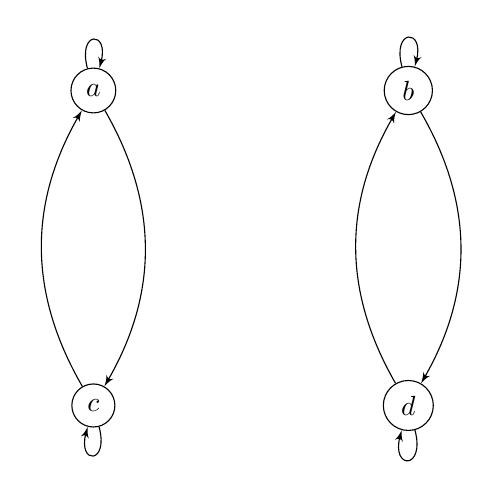
\begin{tikzpicture}
            % Vertices
            \node[vertex] (a) at (0,0) {$a$};
            \node[vertex] (b) at (4,0) {$b$};
            \node[vertex] (c) at (0,-4) {$c$};
            \node[vertex] (d) at (4,-4) {$d$};

            % Edges
            % a
            \draw[edge] (a) to[loop above] (a);
            \draw[edge] (a) to[bend left] (c);

            % b 
            \draw[edge] (b) to[loop above] (b);
            \draw[edge] (b) to[bend left] (d);

            % c
            \draw[edge] (c) to[bend left] (a);
            \draw[edge] (c) to[loop below] (c);

            % d 
            \draw[edge] (d) to[bend left] (b);
            \draw[edge] (d) to[loop below] (d);
        \end{tikzpicture}
    \end{figure}
    \pagebreak
    \section*{Problem 5}
    A Lemma in the book states: {\em Let $A$ be a set with $n$ elements, and let $R$ be a relation on $A$. If there is a path of length at least one in $R$ from $a$ to $b$, then there is such a path with length not exceeding $n$. Moreover, when $a \neq b$, if there is a path of length at least one in R from a to b, then there is such a path with length not exceeding $n-1$}. The book proves for the case that $a=b$. Find the proof for the case that $a \neq b$.
    \subsection*{Solution}
    \pagebreak
    \section*{Problem 6} \label{question}
    Draw the directed graph that represents the relation: 
    \[ A \rel A=\{( a, a), ( a, b), ( b, c), ( c, b), ( c, d), ( d, a), ( d, b)\} \]
    where $A=\{a, b,c,d,e\}$
    \subsection*{Solution}
    \begin{figure}[H]
        \centering
        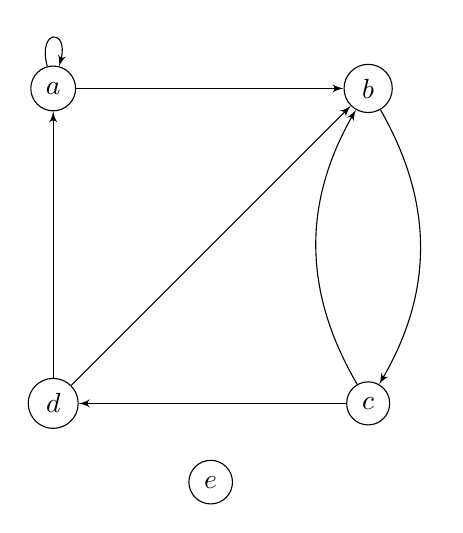
\begin{tikzpicture}
            % Vertices
            \node[vertex] (a) at (0,0) {$a$};
            \node[vertex] (b) at (4,0) {$b$};
            \node[vertex] (c) at (4,-4) {$c$};
            \node[vertex] (d) at (0,-4) {$d$};
            \node[vertex] (e) at (2,-5) {$e$};

            % Edges
            % a
            \draw[edge] (a) to[loop above] (a);
            \draw[edge] (a) to (b);
            
            % b
            \draw[edge] (b) to[bend left] (c);

            % c
            \draw[edge] (c) to[bend left] (b);
            \draw[edge] (c) to (d);

            % d
            \draw[edge] (d) to (a);
            \draw[edge] (d) to (b);
        \end{tikzpicture}
    \end{figure}
    \pagebreak
    \section*{Problem 7}
    Find the matrix of the relation of $A \rel A$  from \hyperref[question]{Question 6} above.
    \subsection*{Solution}
    \[ M = \begin{bmatrix}
        1 & 0 & 0 & 1 & 0 \\
        1 & 0 & 1 & 1 & 0 \\
        0 & 1 & 0 & 0 & 0 \\
        0 & 0 & 1 & 0 & 0 \\ 
        0 & 0 & 0 & 0 & 0 \\
    \end{bmatrix} \]
    \pagebreak
    \section*{Problem 8}
    From the directed graph of  question \hyperref[question]{Question 6} above draw the digraph of $\bar{R}$ (the complement of $R$).
    \subsection*{Solution}
    \[ \overline{M} = \begin{bmatrix}
        0 & 1 & 1 & 0 & 1 \\
        0 & 1 & 0 & 0 & 1 \\
        1 & 0 & 1 & 1 & 1 \\
        1 & 1 & 0 & 1 & 1 \\
        1 & 1 & 1 & 1 & 1 \\
    \end{bmatrix} \]
    \begin{figure}[H]
        \centering
        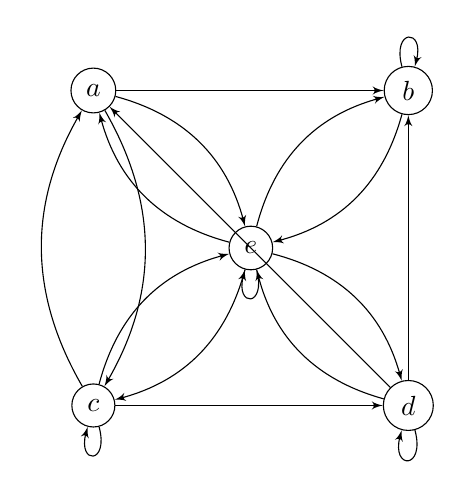
\begin{tikzpicture}
            % Vertices
            \node[vertex] (a) at (0,0) {$a$};
            \node[vertex] (b) at (4,0) {$b$};
            \node[vertex] (c) at (0,-4) {$c$};
            \node[vertex] (d) at (4,-4) {$d$};
            \node[vertex] (e) at (2,-2) {$e$};

            % Edges
            % a
            \draw[edge] (a) to (b);
            \draw[edge] (a) to[bend left] (c);
            \draw[edge] (a) to[bend left] (e);

            % b
            \draw[edge] (b) to[loop above] (b);
            \draw[edge] (b) to[bend left] (e);

            % c
            \draw[edge] (c) to[bend left] (a);
            \draw[edge] (c) to[loop below] (c);
            \draw[edge] (c) to (d);
            \draw[edge] (c) to[bend left] (e);

            % d
            \draw[edge] (d) to (a);
            \draw[edge] (d) to (b);
            \draw[edge] (d) to[loop below] (d);
            \draw[edge] (d) to[bend left] (e);

            % e
            \draw[edge] (e) to[bend left] (a);
            \draw[edge] (e) to[bend left] (b);
            \draw[edge] (e) to[bend left] (c);
            \draw[edge] (e) to[bend left] (d);
            \draw[edge] (e) to[loop below] (e);
        \end{tikzpicture}
    \end{figure}
    \pagebreak
    \section*{Problem 9}
    From the directed graph of question \hyperref[question]{Question 6} above draw the digraph of $R^{-1}$ (the inverse of $R$).
    \subsection*{Solution}
    \pagebreak
    \section*{Problem 10}
    Find the matrix of the relation of $A{\bar R}A$  from question \hyperref[question]{Question 6} above.
    \subsection*{Solution}
    \pagebreak
    \section*{Problem 11}
    Find the matrix of the relation of $A \rel^{-1}A$ from question \hyperref[question]{Question 6} above.
    \subsection*{Solution}
    \pagebreak
    \section*{Problem 12}
    In $A \rel A$ from question \hyperref[question]{Question 6} above remove or add the least amount of  elements so that $A \rel A$ represents an equivalence relation.
    \subsection*{Solution}
\end{document}
